%!TEX root = ../master.tex
\section{Semantic Web and RDF}
In general semantic web and semantic web technologies is an extension of World Wide Web,
but it dosen't refer to one concrete extension. The goal for the semantic web is to make is to 
make the data that are excesibal on the Internet readable for machine. The main way that the semantic web 
dose this is ot have \textit{linked date} which refers to that the identifiers are pointers to Web addresses 
where we can find more information about hte object.
The data that are conected needs som formal semanitc to work, e.g. RDF, RDFS, OWL etc. These components, shown in figure \nameref{fig:SW stack}
are used to among other things structure the linked data by providing a formal description
of terms, relationships and concept in the knowledge domain. In semanitc web and computer science in general 
we would call this an \textbf{ontologi}, which in short can be defined as the knowledge we have about a given 
domain which is machine-prosecassable and with a formally defined meaning.

\begin{figure}
    \centering
    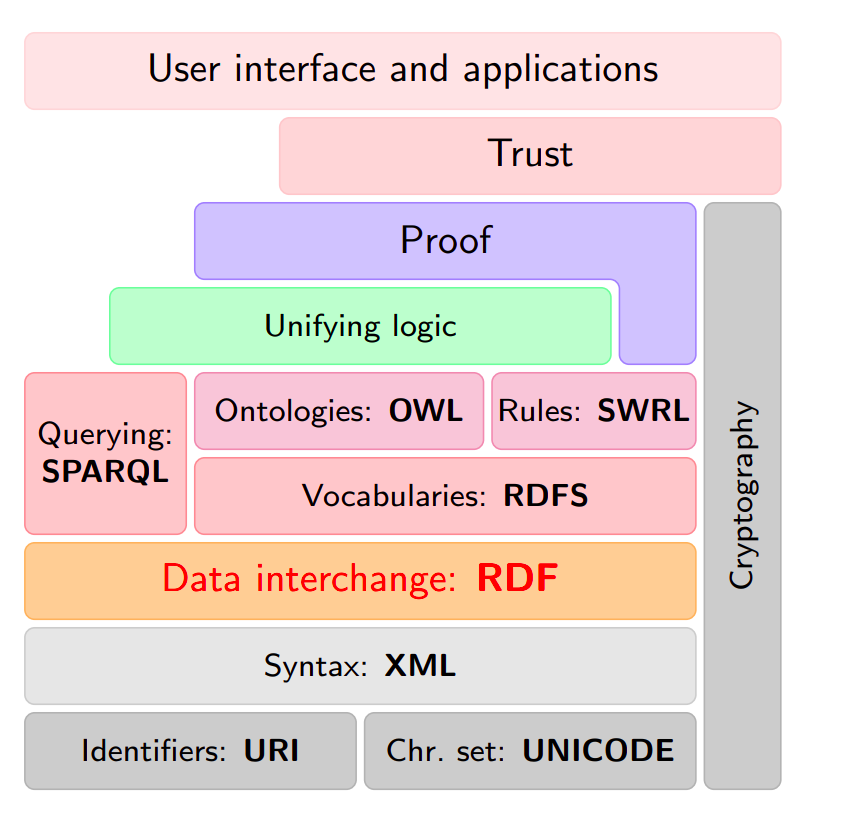
\includegraphics[scale=0.2]{SWStack.png}
    \caption{The semantic web stack src: IN3060 foiler uke 2}
    \label{fig:SW stack}
\end{figure}


\subsection{RDF}
RDF stands for Resource Description Framework and it is a language for formally describing structure data, 
and is the general method in semantic web for describing information that is in a web resource. An RDF document describes 
a directed graph which is build up by tripls which again are build up from subject predicate and object. This is a relation 
from the subject to the object where the predicate tells ous about what the relationship is. In the grap the object 
and subject will be represented as node, with the predicate as an directed edge between the two from the subject to the predicate.
An collection of several will then result in a directed graph. An exampel of an triple can be that Sebastian hasFather Thommas, where 
Sebastian is the object, hasFather is the predicate and Thommas is the object. RDF have several serializations, we will use Turlte for exampels. 
\\ \\
To make this system work we somehow need to uniquely identify the different resources (subject, predicate and objects) of the graph, 
and this is called \textbf{URIs} (Uniform Resource Locators). Every URL is an URI ($URL\subseteq URI$), but it's important to note that 
not all URIs are URL ($URL\nsubseteq URI$). So if we now want to make the tripel made earlier we need to write it out with full URI, that could look 
some thing like this \textit{http://example.org/person/Sebeastian http://example.org/relation/hasFather http://example.org/person/Thommas}
But it can be time consuming to write the whole URI for Sebastian every time we whant to refer to the Sebastian resource, therefore we have something called prefix in 
turtle. We need to set the prefixes in the start of the file with this syntax \textit{@PREFIX ex-p: <http://example.org/person/> .} when we want 
to use the Sebastian resource we can just write $ex-p:Sebastian$. If we now add the the prefix for /relation as well \textit{@PREFIX ex-r: <http://example.org/relation/> .} 
the triple can be written as $ex-p:Sebastian\; ex-r:hasFather\; ex-p:Thommas\; .$.
\\ \\ 
In the ontologi of family, which we have now started to model, it could be nice to express that Sebastian has a father, without us knowing who the father is. 
This can be done with a \textbf{blank node}. In rdf a blank node tells ous that we don't know the URI for the resource, but that we either have some information 
on it or that some other resource is conected to it via a predicate, it is important to note that a blank not can be in the predicate position only in the subject and object
position. So to model that Sebastian has a father we can write either $ex-p:Sebastian\; ex-r:hasFather\; \_:b .$ or $ex-p:Sebastian\; ex-r:hasFather\; [\; ]$ , since the syntax 
for writing an empty node in turtle is either $\_:<some variable name>$ or $[\; ]$. Since an empty node also can be an subject we can express things about the resources. If we 
f.eks. want to model that Sebastian has a father which has a father how is http://example.org/person/Roger we can write $ex-p:Sebastian\; ex-r:hasFather\; [\; ex-r:hasFather\; ex-p:Roger]$
\\ \\ 
In RDF we also have something called literls for expressing stirngs, integer, etc. Literals can only be in the object position of the triple. 
So if we want to express that Sebastian has age 21 we can write $ex-p:Sebastian\; ex-r:hasAge\; " 22 " <opp greie> <opp greie> xsd:int.$ where xsd comes from the prefix
$@prefix\; xsd:\; <http://www.w3.org/2001/XMLSchema\#> .$. We can also model that Sebastian has the name Sebastian in norwiagen and Bastian in english by using 
language tags, this gives use the triples $ex-p:Sebastian\; ex-r:hasName\; Sebastian@no.$ and $ex-p:Sebastian\; ex-r:hasName\; Bastian@en.$. Here har our full 
graph:
\\ \\

\begin{lstlisting}[frame=single, language=turtle]
    @prefix  ex-p:  <http://example.org/person/> . 
    @prefix ex-r:  <http://example.org/relation/> . 
    @prefix xsd: <http://www.w3.org/2001/XMLSchema\#>  . 
    ex-p:Sebastian ex-r:hasFather ex-p:Thommas .
    ex-p:Sebastian ex-r:hasFather [ ex-r:hasFather ex-p:Roger] . 
    ex-p:Sebastian ex-r:hasAge  "22"^^xsd:int . 
    ex-p:Sebastian ex-r:hasName  Sebastian@no . 
    ex-p:Sebastian ex-r:hasName  Bastian@en .
\end{lstlisting}
In addition to the abbreviations we have already made turtle stile have some more abbreviations when writing the triples. For instanse if we have the same 
predicate and subject several times, with different objects, we can just write the predicate and subject one time and seperate the objects with a ,. Futhermore 
we can also abbreviate when we use the same subject severalt times by writne ; in the end of the line instead of . . This gives this turtle file:
\\ \\
\begin{lstlisting}[frame=single, language=turtle]
    @prefix  ex-p:  <http://example.org/person/> . 
    @prefix ex-r:  <http://example.org/relation/> . 
    @prefix xsd: <http://www.w3.org/2001/XMLSchema\#>  . 
    ex-p:Sebastian ex-r:hasFather ex-p:Thommas, [ ex-r:hasFather ex-p:Roger] ; 
                   ex-r:hasAge  "22"^^xsd:int ; 
                   ex-r:hasName  Sebastian@no, Bastian@en ;
\end{lstlisting}

Figure \refname{fig:exampelGraph} is a visual graph of the graph we just made.
\begin{figure}
    \centering
    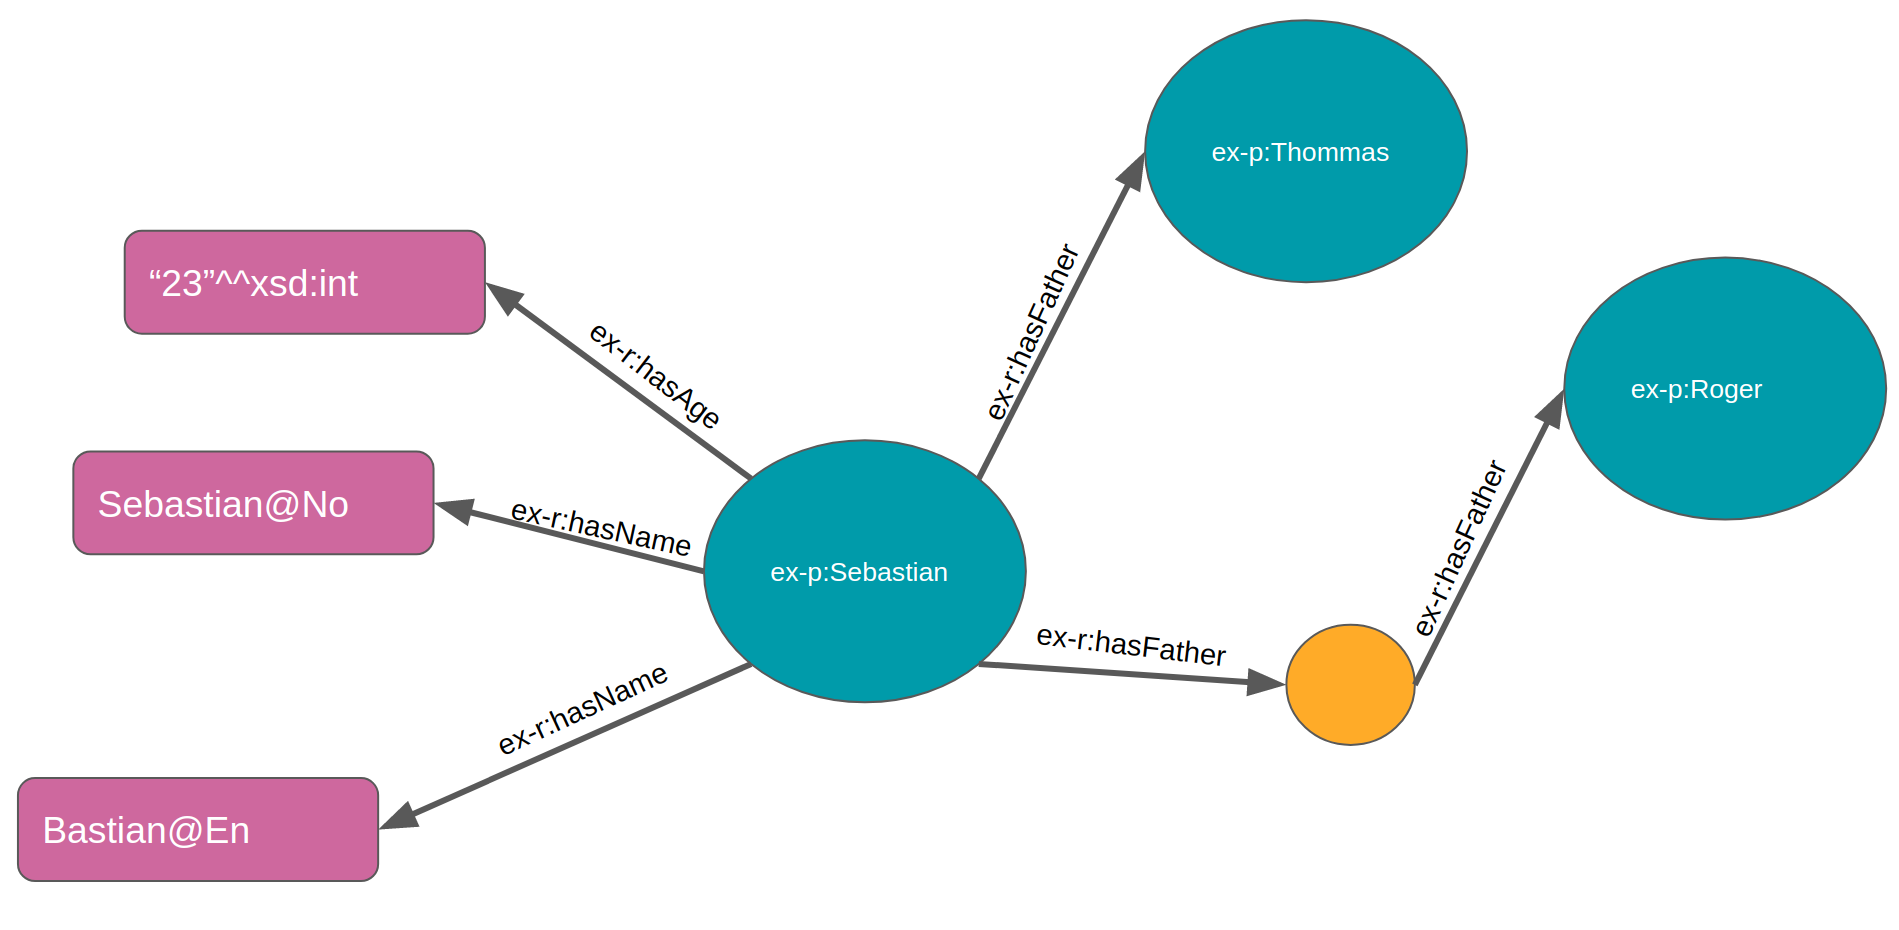
\includegraphics[scale=0.2]{exampleGraph.png}
    \caption{The visual graph over the graph made in section 2.1}
    \label{fig:exampelGraph}
\end{figure}




\begin{itemize}
    \item Kort om historien til SW og SWT 
    \begin{itemize}
        \item extension av WWW
        \item Data requires formal semantics
        \item goal: Machine can access more information
    \end{itemize}
    \item Snakke om ontologies, fra oppsumering i boka + eksempler: 
    \textit{Ontology}: The study of existence and being as such, and of the fundamental 
    classes and relationships of existing things. \textbf{In computer scienence} an ontologi 
    is a description of knowledge about a domain of interest, the core of which is a 
    machine-processable specification with a formally defined meaning
    \item RDF (bruker turtle syntax ?)
    \begin{itemize}
        \item hvordan det er bygd opp: object predicate subject
        \item at det er et formelt språk for å forklare strukturert data 
        \item Er en graph, og kan bli sett på som en directed graph.
        \item Kort om URI, bruk av prefix
        \item Literals
        \item Blank nodes
    \end{itemize}
    \item Å lage mer kompliserte strukturer over RDF
    \item Skrive om ottr, type systemet og hvilke mangler det har. Kanskje mangler 
    burde komme sammen med den delen hvor man forklarer oppbygning av funksjonen.
\end{itemize}
